\id{МРНТИ 62.09.37}{https://doi.org/10.58805/kazutb.v.2.27-1047}

\begin{articleheader}
\sectionwithauthors{А.Н. Құрманәлі, Ш.А. Абжанова, Л.К. Байболова, М.К. Алимарданова, М.Серікқызы}{ШЫРҒАНАҚ СЫҒЫНЫНАН АЛЫНҒАН ЭКСТРАКТ ҚОСЫЛҒАН ЖЫЛҚЫ ЕТІНІҢ ҚҰРАМЫН ЗЕРТТЕУ}

{\bfseries
\textsuperscript{1}А.Н. Құрманәлі\alink{https://orcid.org/0009-0004-8118-1321}\textsuperscript{\envelope},
\textsuperscript{1}Ш.А. Абжанова\alink{https://orcid.org/0000-0003-3209-6855},
\textsuperscript{2}Л.К. Байболова\alink{https://orcid.org/0000-0002-8118-1581},
\textsuperscript{1}М.К. Алимарданова\alink{https://orcid.org/0000-0003-4861-7862},
\textsuperscript{1}М.~Серікқызы\alink{https://orcid.org/0000-0002-1653-9890}
}
\end{articleheader}

\begin{affiliation}
\textsuperscript{1}Алматы технологиялық универсиеті, Алматы, Қазақстан,

\href{https://www.kaztbu.edu.kz/}{\textsuperscript{2}Қ.Құлажанов атындағы қазақ технология және бизнес университеті}

\raggedright \textsuperscript{\envelope }Корреспондент-автор: aktoty.kurmanali@mail.ru
\end{affiliation}

Бұл зерттеу жұмысында шырғанақ (\emph{Hippophae rhamnoides}) сығынынан
алынған табиғи экстрактыны жылқы етіне, нақтырақ айтқанда қазақ халқының
дәстүрлі ұлттық тағамы - жаяға қосу арқылы алынған дайын өнімнің
физика-химиялық және биохимиялық сипаттамаларына әсері жан-жақты
қарастырылды. Жая - жылқының сан етінен дайындалатын, дәмдік, құнарлық
және тағамдық сапасы жоғары бағаланатын өнім. Оның құрамында ақуыз,
темір, С және Е дәрумендері секілді адам ағзасына пайдалы заттар мол
кездеседі.Соңғы жылдары тағам өнеркәсібінде синтетикалық қоспалар мен
консерванттарға балама ретінде табиғи өсімдік тектес компоненттерді
қолдану үрдісі кең етек алып келеді. Бұл бағытта шырғанақ өсімдігі
ерекше назарға ілініп отыр. Себебі шырғанақ құрамында каротиноидтар,
флавоноидтар, фенолды қосылыстар, С және Е дәрумендері, сондай-ақ
биологиялық белсенді заттар молынан кездеседі. Мұндай заттар ет
өнімдерінің тотығуға қарсы тұрақтылығын арттырып, олардың сақтау
мерзімін ұзартады, тағамдық және функционалдық қасиеттерін жақсартады.
Жұмыста шырғанақ экстрактысы әртүрлі концентрацияда жая етіне қосылып,
алынған үлгілер физика-химиялық және биохимиялық көрсеткіштері бойынша
салыстырылды. Бұл нәтижелер шырғанақ экстрактысын қосу ет өнімінің тек
тағамдық құндылығын ғана емес, оның сақтау қасиеттерін де айтарлықтай
жақсартатынын көрсетті. Сонымен қатар, мұндай тәсіл функционалдық және
байытылған тағам түрлерін жасауға жаңа мүмкіндіктер береді. Бұл әсіресе
денсаулықты сақтауға бағытталған тағам өндіру саласында ерекше маңызға
ие.Зерттеу нәтижелері шырғанақ экстрактысын ет өнімдеріне енгізу ---
тамақ өнеркәсібінің инновациялық бағыты ретінде болашағы зор екендігін
дәлелдеді. Алынған мәліметтер отандық азық-түлік қауіпсіздігін
қамтамасыз етуге, сондай-ақ ұлттық тағам өнімдерін жаңа деңгейге
көтеруге септігін тигізеді.

{\bfseries Түйін сөздер:} Жая, жылқы еті, шырғанақ сығыны, экстракт,
антиоксиданттар, тағамдық құндылық, функционалдық өнімдер.

\begin{articleheader}
{\bfseries ИССЛЕДОВАНИЕ СОСТАВА МЯСА КОНИНЫ С ДОБАВЛЕНИЕМ ЭКСТРАКТА ЖМЫХА ОБЛЕПИХИ}

{\bfseries
\textsuperscript{1}А.Н. Курманали\textsuperscript{\envelope },
\textsuperscript{1}Ш.А. Абжанова,
\textsuperscript{2}Л.К. Байболова,
\textsuperscript{1}М.К. Алимарданова,
\textsuperscript{1}М. Сериккызы
}
\end{articleheader}

\begin{affiliation}
\textsuperscript{1}Алматинский технологический университет, Алматы, Казахстан,

\textsuperscript{2}Казахский университет технологий и бизнеса им.~К.Кулажанова, Алматы, Казахстан,

e-mail: aktoty.kurmanali@mail.ru
\end{affiliation}

В данной исследовательской работе было всесторонне рассмотрено влияние
природного экстракта из жмыха облепихи (\emph{Hippophae rhamnoides}) на
физико - химические и биохимические характеристики готового продукта,
полученного путем добавления его в конину, а точнее в жая традиционное
национальное блюдо казахского народа. Жая-продукт, изготавливаемый из
мяса конского бедра, который высоко ценится за вкусовые, питательные и
питательные качества. В его составе много полезных для организма
человека веществ, таких как белок, железо, витаминыС и Е. В последние
годы в пищевой промышленности набирает обороты тенденция использования
натуральных растительных компонентов в качестве альтернативы
синтетическим добавкам и консервантам. В этом направлении особого
внимания заслуживает облепиха. Это связано с тем, что облепиха содержит
большое количество каротиноидов, флавоноидов, фенольных соединений,
витаминов С и Е, а также биологически активных веществ. Такие вещества
повышают антиокислительную устойчивость мясных продуктов, продлевают
срок их хранения, улучшают пищевые и функциональные свойства. В работе
экстракт облепихи соединяли с растительным мясом в различных
концентрациях, а полученные образцы сравнивали по физико-химическим и
биохимическим показателям. Эти результаты показали, что добавление
экстракта облепихи значительно улучшает не только пищевую ценность
мясного продукта, но и его сохраняющие свойства. Кроме того, такой
подход дает новые возможности для создания функциональных и обогащенных
видов пищи. Это особенно важно в области производства продуктов питания,
которая направлена на сохранение здоровья. Результаты исследования
доказали, что внедрение экстракта облепихи в мясную продукцию является
перспективным инновационным направлением пищевой промышленности.
Полученные данные помогут обеспечить отечественную продовольственную
безопасность, а также вывести национальные продукты питания на новый
уровень.

{\bfseries Ключевые слова:} Жая, конина, жмых облепихи, экстракт,
антиоксиданты, пищевая ценность, функциональные продукты.

\begin{articleheader}
{\bfseries STUDY OF THE COMPOSITION OF HORSE MEAT WITH THE ADDITION OF SEA BUCKTHORN PRESS CAKE EXTRACT}

{\bfseries
\textsuperscript{1}A.N. Kurmanali\textsuperscript{\envelope },
\textsuperscript{1}Sh.A. Abzhanova,
\textsuperscript{2}L.K. Baibolova,
\textsuperscript{1}M.K. Alimardanova,
\textsuperscript{1}M. Serikkyzy
}
\end{articleheader}

\begin{affiliation}
\textsuperscript{1}Almaty Technological University, Almaty, Kazakhstan

\textsuperscript{2}Kazakh University of Technology and Business named after K.Kulazhanov, Almaty, Kazakhstan,

e-mail: aktoty.kurmanali@mail.ru
\end{affiliation}

In this research paper, the effect of a natural extract from sea
buckthorn press cake (\emph{Hippophae rhamno\-ides}) on the
physico-chemical and biochemical characteristics of the finished product
obtained by adding it to horsemeat, or rather to zhaya, a traditional
national dish of the Kazakh people, was comprehensively considered.
Zhaya is a product made from horse thigh meat, which is highly
appreciated for its taste, nutritional and nutritional qualities. It
contains many substances useful for the human body, such as protein,
iron, vitamins C and E. In recent years, the trend of using natural
herbal ingredients as an alternative to synthetic additives and
preservatives has been gaining momentum in the food industry. Sea
buckthorn deserves special attention in this area. This is due to the
fact that sea buckthorn contains a large amount of carotenoids,
flavonoids, phenolic compounds, vitamins C and E, as well as
biologically active substances. Such substances increase the antioxidant
resistance of meat products, prolong their shelf life, and improve
nutritional and functional properties. In the work, sea buckthorn
extract was combined with vegetable meat in various concentrations, and
the samples obtained were compared according to physico-chemical and
biochemical parameters. These results showed that the addition of sea
buckthorn extract significantly improves not only the nutritional value
of the meat product, but also its preserving properties. In addition,
this approach provides new opportunities for creating functional and
enriched types of food. This is especially important in the field of
food production, which is aimed at maintaining health. The results of
the study proved that the introduction of sea buckthorn extract into
meat products is a promising innovative area of the food industry. The
data obtained will help ensure domestic food security, as well as bring
national food products to a new level.

{\bfseries Keywords:} Zhaya, horsemeat, sea buckthorn press cake, extract,
antioxidants, nutritional value, functi\-onal products.

\begin{multicols}{2}
{\bfseries Кіріспе.} Қазіргі таңда халықтың дұрыс тамақтануына және
функционалдық тағам өнімдерін өндіруге деген сұранысы артып келеді.
Осыған байланысты құрамында биологиялық белсенді заттары бар табиғи
ингредиенттерді қолдану - тағам өнеркәсібінің өзекті бағыттарының біріне
айналуда. Атап айтқанда, өсімдік тектес шикізаттар -- витаминдерге,
антиоксиданттарға, минералдарға және басқа да функционалдық
компоненттерге бай болғандықтан, ет өнімдерінің тағамдық құндылығын
арттыруда маңызды рөл атқарады {[}1{]}.

Жылқы еті - қазақ халқының дәстүрлі азық-түлігінің бірі, ақуызға бай,
оңай қорытылады және аллергиялық реакциялар туғызбайды. Оның құрамында B
тобының дәрумендері, темір мен фосфор секілді микроэлементтер мол
мөлшерде кездеседі {[}2{]}. Сонымен қатар, жая -- жылқы етінің арнайы
тұздап, сүрлеп немесе қақтап дайындалатын жоғары құнарлы және ұзақ
сақтауға жарамды ұлттық тағамы. Жаяның құрылымы тығыз, дәмдік қасиеті
жоғары әрі құрамында май мен ақуыз мөлшері мол {[}3{]}.

Соңғы жылдары ет өнімдеріне табиғи өсімдік тектес экстракттарды, оның
ішінде шырғанақ \emph{(Hippophae rhamnoides L.)} экстрактын қосу арқылы
олардың функционалдық қасиеттерін жақсарту жолдары зерттелуде. Шырғанақ
- құрамында Е, С, А дәрумендері, β-каротин, органикалық қышқылдар мен
флавоноидтар көп мөлшерде кездесетін дәрілік өсімдік {[}4{]}. Одан
алынған экстракттар антиоксиданттық, қабынуға қарсы, иммунитетті
нығайтатын әсерге ие. Осы қасиеттер шырғанақ сығындысын ет өнімдерінде
қолдануға мүмкіндік береді {[}5{]}.

Зерттеу жұмысының мақсаты- шырғанақ сығымынан алынған экстрактты жая
(жылқы еті) құрамына қосу арқылы оның физика-химиялық және биохимиялық
қасиеттерінің өзгерісін зерттеу, сонымен қатар өнімнің тағамдық және
функционалдық құндылығын арттыру жолдарын анықтау.

{\bfseries Материалдар мен әдістер}.Зерттеу жұмысына негізгі шикізат
ретінде жылқы етінен дайындалған жая жәнешырғанақ сығымынан алынған
экстракт пайдаланылды. Зерттелетін өнім бірқатар физика-химиялық және
биохимиялық көрсеткіштер бойынша талдаудан өтті. Атап айтқанда:
ылғалдың, ақуыздың, майдың, көмірсулардың, күлдің, сондай-ақ
витаминдердің, минералды элементтердің және антиоксиданттардың массалық
үлесі анықталды. Барлық зерттеу жұмыстары қолданыстағы мемлекеттік
стандарттар мен әдістемелік нұсқаулықтарға сәйкес жүргізілді .

Ылғал мөлшері кептіргіш шкафында 105°C температурада тұрақты массаға
дейін кептіру әдісімен анықталды {[}6{]}. Үлгінің бастапқы және соңғы
массасы арасындағы айырмашылыққа негізделіп, ылғалдың массалық үлесі
жалпы массаға пайызбен есептелді. Ақуыз мөлшері Кьельдаль әдісімен
анықталды {[}7{]}. Үлгі алдын ала кептіріліп, кейін күкірт қышқылында
қорытылып, бейтараптандырылып, титрлеу арқылы азот мөлшері есептелді.
Азот негізінде ақуыз мөлшері пайызбен белгіленді. Май мөлшері
органикалық еріткішпен экстракциялау арқылы анықталды {[}8{]}. Еріткіш
ретінде мұнай эфирі қолданылды. Май ерітіндіден бөлініп, кептірілген
соң, оның массасы құрғақ заттың жалпы массасына қатысты пайызбен
есептелді. Көмірсу мөлшері перманганометриялық әдіспен анықталды
{[}9{]}. Бұл әдіс көмірсуларды калий перманганаты арқылы тотықтыру және
артық титрленетін перманганат көлеміне қарай мөлшерін анықтауға
негізделген. Күлдің мөлшері үлгіні 550°C шамасында жоғары температурада
жағу арқылы есептелді {[}10{]}. Барлық органикалық заттар жойылғаннан
кейін қалған бейорганикалық қалдықтың массасы пайызбен белгіленді. Е
дәрумені жоғары тиімді сұйық хроматография әдісімен анықталды {[}11{]}.
Токоферолдар органикалық еріткішпен экстракцияланып, хроматографиялық
жүйеде сандық түрде өлшенді. С дәрумені титриметриялық әдіспен, яғни
йодпен тотығу және артық мөлшерін тиосульфатпен титрлеу арқылы анықталды
{[}12{]}. Антиоксиданттар мөлшері амперометриялық әдіспен анықталды
{[}13{]}. Белгілі бір потенциалда электрод бетінде заттардың тотығу
кезінде пайда болған ток күші өлшеніп, стандартты кверцетинмен
салыстырылды. Минералды элементтер мырыш, мыс және магний мөлшері
атомды-абсорбциялық спектрометрия әдісімен анықталды. Алдымен үлгілер
тұз қышқылында ерітіліп, қажет болған жағдайда алдын ала күлдендірілді.
Алынған ерітінді ацетилен-ауа жалынында атомизацияланып, элементтердің
сіңіру қарқындылығы арқылы мөлшері есептелді.

{\bfseries Нәтижелер және талқылау.} 1- кестеде жая етіне 5\%, 7\% және 9\%
мөлшерінде шырғанақ сығынынан алынған экстракт қосылғаннан кейінгі
негізгі физика-химиялық көрсеткіштердің өзгерісін көрсетеді. Нәтижелер
бақылау үлгісімен салыстырғанда айтарлықтай оң өзгерістерді көрсетті.
Ылғал мөлшері шырғанақ экстракты қосылған сайын сәл артқаны байқалады,
бұл өнімнің ылғал сақтағыштық қасиетін жақсартуы мүмкін екенін
көрсетеді.Ақуыз мөлшері барлық үлгілерде едәуір жоғарылаған, бұл
шырғанақ сығындысының құрамындағы биологиялық белсенді қосылыстардың
ақуыз биосинтезін арттыратындығымен байқауға болады.
\end{multicols}

\tcap{1 - кесте. Жая етіне шырғанақ сығындысының әртүрлі концентрацияларын қосқаннан кейінгі физика-химиялық көрсеткіштерінің өзгерісі}
\begin{longtblr}[
  label = none,
  entry = none,
]{
  width = \linewidth,
  colspec = {Q[254]Q[179]Q[167]Q[167]Q[167]},
  cells = {c},
  hlines,
  vlines,
}
\textbf{Көрсеткіш} & \textbf{Бақылау			үлгісі} & \textbf{5\%			экстракт} & \textbf{7\%			экстракт} & \textbf{9\%			экстракт}\\
Ылғалдың
			массалық
			үлесі, \% & 65,2 ± 0,82 & 67,8 ± 0,82 & 68,9 ± 0,42 & 67,3 ± 0,42\\
Ақуыздың
			массалық
			үлесі, \% & 21,2 ± 0,79 & 25,44 ± 0,79 & 29,02 ± 0,33 & 29,5 ± 0,33\\
Майдың
			массалық
			үлесі, \% & 31,06 ± 0,25 & 33,4 ± 0,25 & 35,7 ± 1,02 & 37,2 ± 1,02\\
Көмірсулардың
			массалық
			үлесі, \% & Табылған
			жоқ & Табылған
			жоқ & Табылған
			жоқ & Табылған
			жоқ\\
Күлдің
			массалық
			үлесі, \% & 5,28 ± 0,06 & 6,01 ± 0,06 & 6,23 ± 0,03 & 6,92 ± 0,03\\
Құрғақ
			заттардың
			массалық
			үлесі, \% & 30,01 ± 0,37 & 35,57 ± 0,37 & 37,8 ± 0,73 & 38,9 ± 0,73
\end{longtblr}

\begin{multicols}{2}
Майдың массалық үлесі де біртіндеп артқан, бұл экстракт құрамындағы
кейбір липидтік компоненттердің өнімге сіңуінен болуы мүмкін.Күл мөлшері
жоғарылағаны -- минералдық құрамның байығанын білдіреді, бұл әсіресе
цинк, мыс, магний сияқты микроэлементтердің өсуімен байланысты. Құрғақ
зат мөлшері де артып, өнімнің тығыздығы мен сақтау тұрақтылығы
жақсарғанын көрсетеді. Көмірсулар анықталмаған, себебі жая еті мен
шырғанақ экстрактының өзінде көмірсу мөлшері өте төмен.

Жаяға шырғанақ сығынынан экстракт қосу нәтижесінде өнімнің сақтау
тұрақтылығына және сапасына әсер ететін көрсеткіштер бойынша
өзгерістерге түсіндірілді. Тиобарбитуралық сан (ТБС), малональдегид бұл
көрсеткіш еттегі майлардың тотығу дәрежесін сипаттайды. ТБС мәнінің
жоғарылауы өнімде тотығу процестерінің жүргенін көрсетеді. Экстракт
концентрациясы артқан сайын ТБС өсіп отыр, бұл шырғанақтың өзінде бар
табиғи антиоксиданттардың шектен тыс концентрацияда кері әсер етуі
немесе тотығуға бейім қосылыстардың көбеюімен түсіндіріледі. Бірақ бұл
көрсеткіш 2 мг/кг-дан аспайтындықтан, санитарлық норма шегінде,
яғни өнім қауіпсіз болып қала береді. Ас тұзының массалық үлесі, дәм мен
сақтау мерзіміне әсер ететін маңызды компонент. Шырғанақ
экстрактысын қосу тұздың жалпы құрамын арттырғанын көрсетеді. Бұл
шырғанақ қалдығында табиғи минералды тұздардың болуы немесе
технологиялық процесте тұз қосудың артуына байланысты деп түсіндірді.
Жоғары тұз мөлшері сақтау мерзімін ұзартады, бірақ дәмнің тым ащы
болмауын ескерілді. Майдың қышқылдық саны бұл көрсеткіш майдың
гидролиздік бұзылу дәрежесін білдіреді.

Қышқылдық саны май құрамындағы бос май қышқылдарының мөлшерін көрсетеді.
Экстракт қосылған үлгілерде бұл көрсеткіш бақылаумен салыстырғанда
біршама төмендеген немесе тұрақты, бұл шырғанақ экстрактысының
құрамындағы антиоксиданттардың майларды гидролизден қорғауға ықпал
еткенін көрсетеді. Майдың пероксидтік саны, пероксид саны майдың
бастапқы тотығу өнімдерінің (гидропероксидтер) мөлшерін көрсетеді. Бұл
мәндер өте төмен жәнерұқсат етілген деңгейде, яғнимай тотығуы
бақылауда. Шырғанақ экстрактысының табиғи антиоксиданттары
майдың тотығу процесін баяулатуға көмектескен болуы мүмкін.
\end{multicols}

\begin{figure}[H]
	\centering
	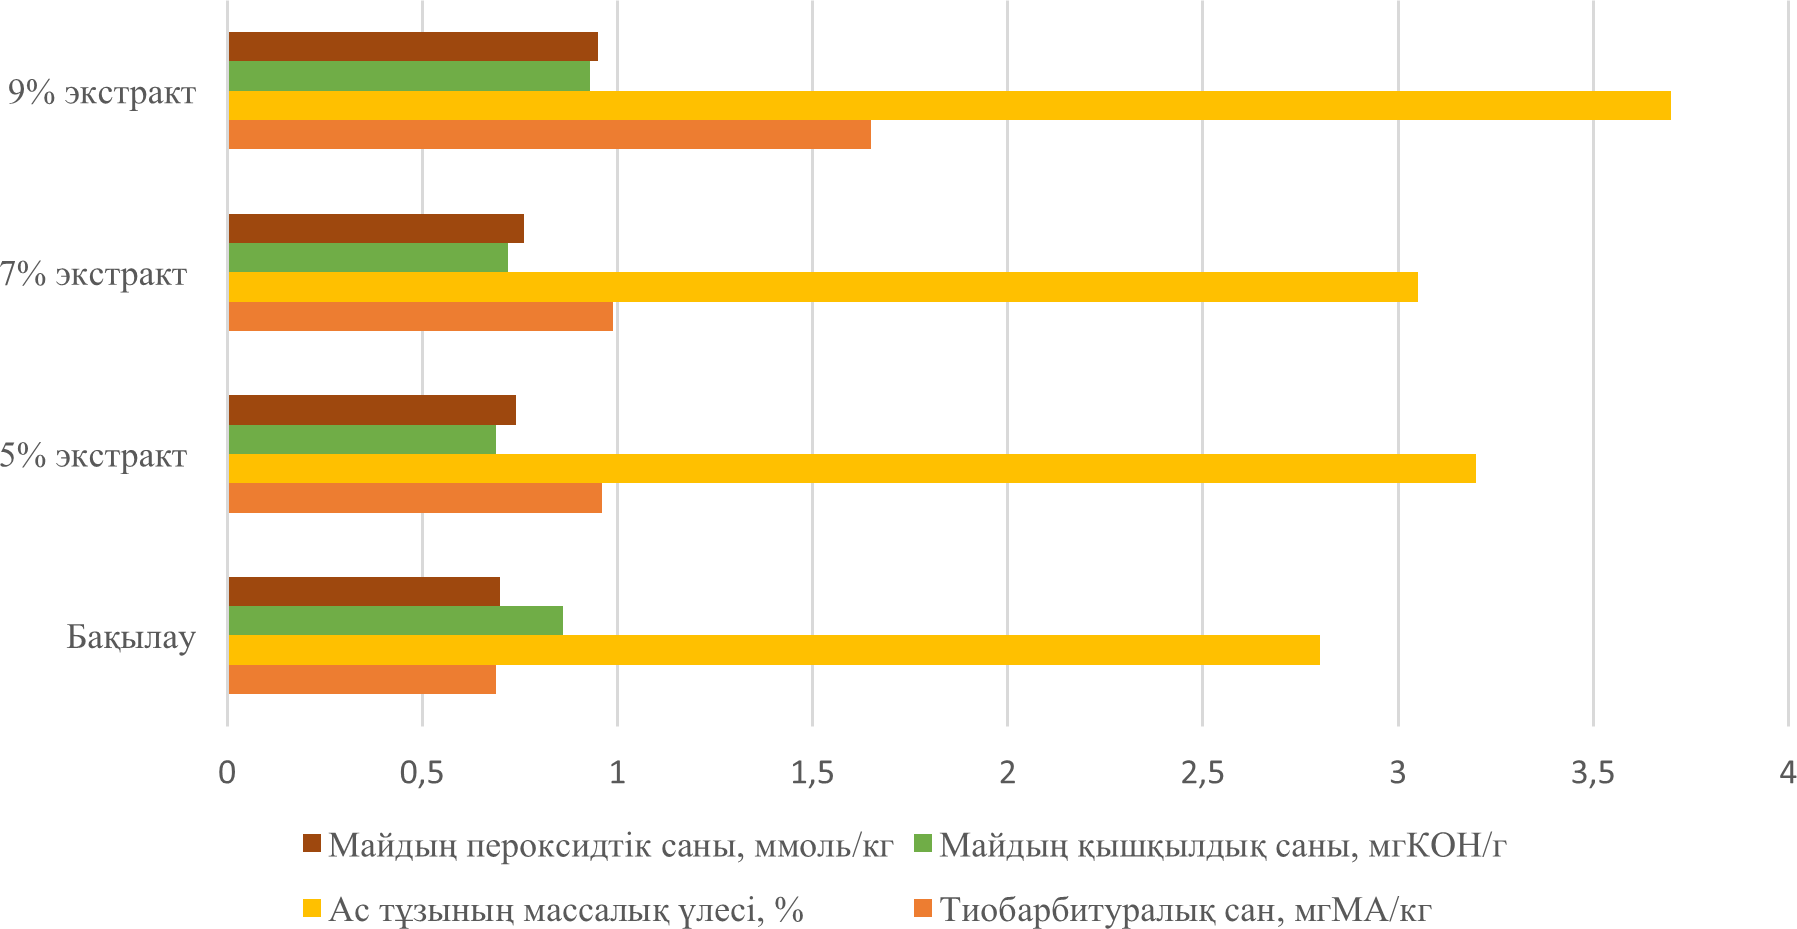
\includegraphics[width=0.8\textwidth]{media/pish4/image2}
	\caption*{1 - сурет. Жая етіне шырғанақ сығымынан алынған экстракты қосу
нәтижесінде өнімнің технологиялық және биохимиялық көрсеткіштері}
\end{figure}

\tcap{2 - кесте. Жая етіне шырғанақ экстрактысын қосу нәтижесінде өнімнің технологиялық көрсеткіштері}
\begin{longtblr}[
  label = none,
  entry = none,
]{
  width = \linewidth,
  colspec = {Q[279]Q[173]Q[160]Q[160]Q[160]},
  cells = {c},
  hlines,
  vlines,
}
\textbf{Көрсеткішатауы} & \textbf{Бақылауүлгісі} & \textbf{5\%			экстракт} & \textbf{7\%			экстракт} & \textbf{9\%			экстракт}\\
Ылғал
			ұстап тұру қабілеті (ВУС), \% & 60,27 ± 0,40 & 67,4 ± 0,40 & 68,15 ± 0,28 & 72,3 ± 0,39\\
Ылғал
			байланыстырғыш
			қабілеті
			(ВСС), \% & 62,8 ± 0,43 & 65,09 ± 0,43 & 69,19 ± 0,37 & 74,4 ± 0,37\\
Май
			ұстап
			тұру
			қабілеті
			(ЖУС), \% & 60,01 ± 0,26 & 65,8 ± 0,26 & 67,1 ± 0,35 & 69,1 ± 0,35
\end{longtblr}

\begin{multicols}{2}
2 - кестеде жая етіне шырғанақ экстрактысын әртүрлі мөлшерде қосу
нәтижесінде өнімнің технологиялық көрсеткіштеріндегі өзгерістерге
түсіндірмеберілген:ылғал ұстап тұру қабілеті 60,27\% → 72,3\% дейін
артқан. Бұл көрсеткіш өнімнің құрамындағы суды ұстау қабілетін
сипаттайды. Шырғанақ экстрактысын қосу нәтижесінде ет құрылымы
тығыздалып, суды байланыстыру қабілеті артқан. Бұл өнімнің шырынды әрі
жұмсақ болуына септігін тигізеді, сондай-ақ технологиялық өңдеу кезінде
ылғалдың жоғалуын азайтады. Ылғал байланыстырғыш қабілеті 62,8\% →
74,4\% дейін өскен. Бұл еттің ылғалды бұлшықет құрылымымен
байланыстыру мүмкіндігі. Экстракт құрамындағы табиғи қосылыстар (мысалы,
пектиндер, фенолдық қосылыстар) еттегі ақуыздармен әрекеттесе отырып,
суды тиімді ұстап қалуға көмектеседі. Бұл өнімнің физикалық тұрақтылығын
жақсартады және кескенде сұйық бөлінуін азайтады. Май ұстап тұру
қабілеті 60,01\% → 69,1\% дейін артқан. Бұл көрсеткіш еттің өз
құрамындағы майды сақтау қасиеті. Шырғанақ экстрактысы маймен өзара
әрекеттесіп, май бөлшектерінің өнімнен бөлініп кетуіне жол бермейді. Бұл
қасиет дайын өнімнің консистенциясын жақсартады, майдың тепе-тең
бөлінуіне ықпал етеді және өнімнің органолептикалық көрсеткіштерін
жақсартты.
\end{multicols}

\begin{figure}[H]
	\centering
	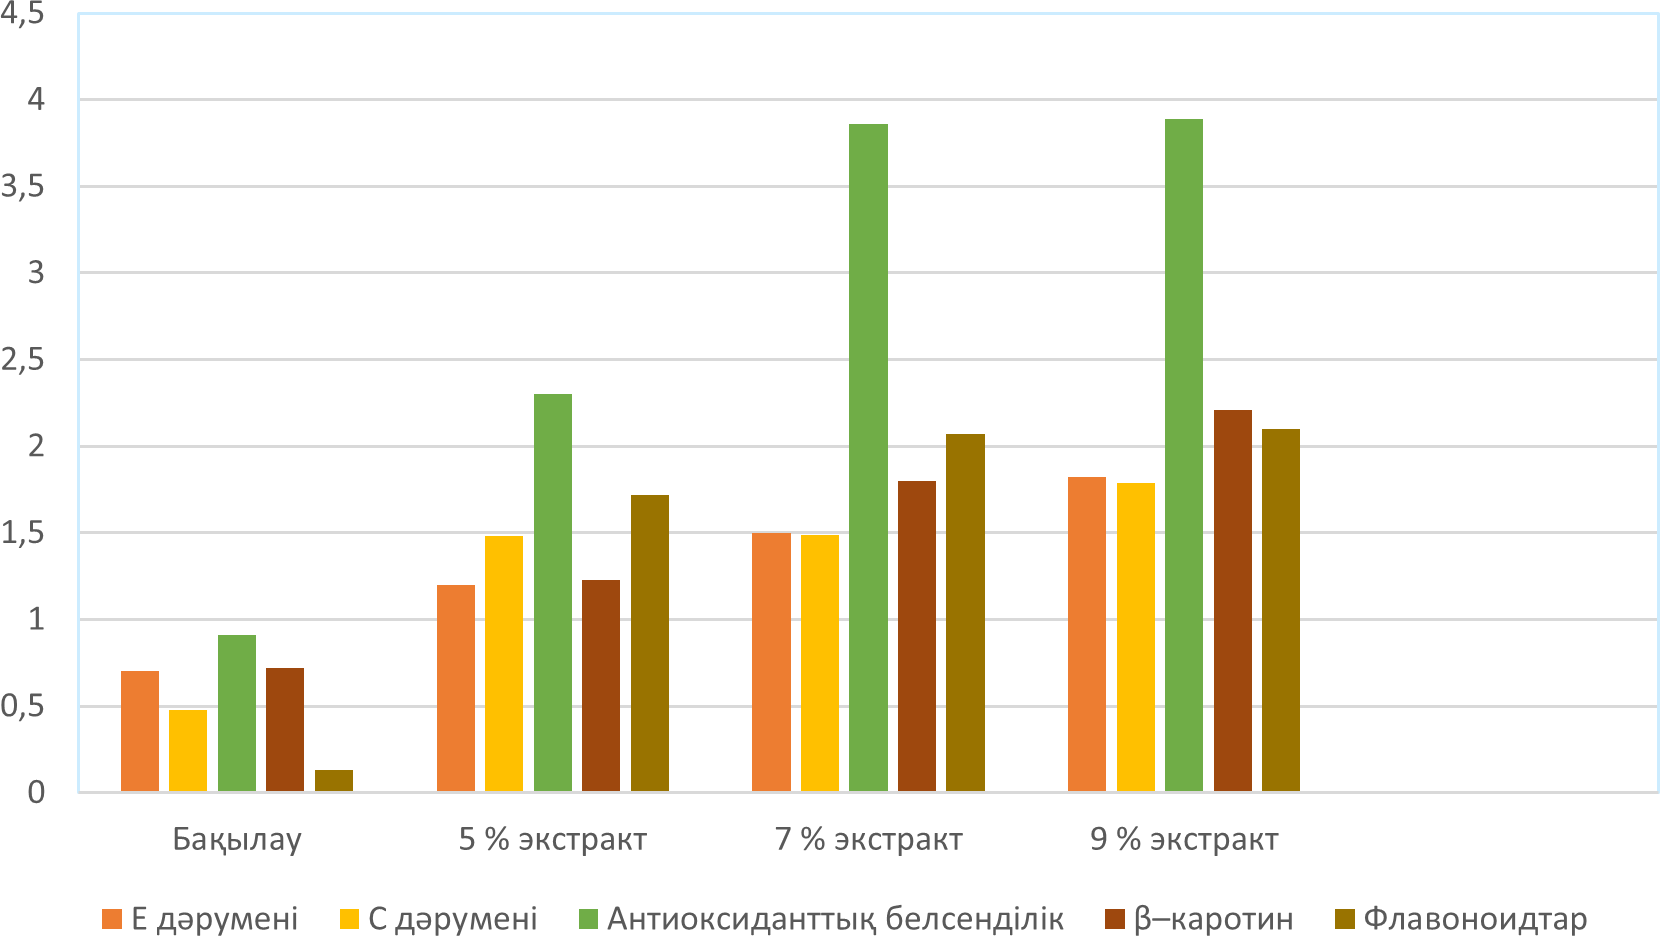
\includegraphics[width=0.8\textwidth]{media/pish4/image3}
	\caption*{2 - сурет. Шырғанақ сығындысы қосылған жая етіндегі биологиялық белсенді заттардың мөлшері}
\end{figure}

\begin{multicols}{2}
2 - сурет бойынша нәтижелері бойынша 7\% экстракт қолданылған үлгіде
антиоксиданттық қосылыстардың айтарлықтай артуы байқалды. Атап айтқанда
Е дәрумені мөлшері бақылаумен салыстырғанда 2,14 есе артып, 1,5 ± 0,16
мг/100 г болды. С дәрумені - 1,49 ± 0,08 мг/100 г, яғни бақылауға
қарағанда 3 есе жоғары. Суда еритін антиоксиданттар - 3,86 ± 0,031 мг/г,
бұл бақылау үлгісінен 4,24 есе артық, β--каротин мөлшері 1,8 ± 0,004
мг/кг құрап, 2,5 есе артты. Флавоноидтар үлесі 2,07 ± 0,008\%, бұл
бақылаумен салыстырғанда шамамен 16 есе жоғары көрсеткіш. Бұл нәтижелер
7\% экстракттың биологиялық белсенді заттармен байытылу жағынан оңтайлы
екенін дәлелдейді. Атап айтқанда, бұл концентрацияда антиоксиданттық
белсенділік жоғары деңгейде, ал 9\% экстрактпен салыстырғанда
айырмашылық мардымсыз. Демек, экстракт мөлшерін 7\% деңгейінде пайдалану
тиімді әрі экономикалық жағынан да ұтымды шешім болып табылады.

{\bfseries Қорытынды.} Шырғанақ сығымынан алынған экстракты қосу арқылы жая
етінің технологиялық қасиеттері едәуір жақсарған. Атап айтқанда, ылғал
мен майды ұстау және байланыстыру қабілеттері артып, өнімнің құрылымдық
тұрақтылығы мен сапалық көрсеткіштері күшейген. Бұл - шырғанақ сығымынан
алынған экстракты табиғи тұрақтандырғыш және құрылым түзуші ретінде
тиімді екенін дәлелдейді.Шырғанақ экстрактысын жая етіне қосу өнімнің
микробиологиялық және тотығу тұрақтылығына оң әсер етеді,
әсіресе майлардың гидролизі мен тотығуынан қорғайды. Зерттеу нәтижелері
көрсеткендей, шырғанақ сығынынан алынған экстрактын 7\% концентрациясы
қосылған жая етінің үлгісі антиоксиданттық белсенділік пен биологиялық
белсенді заттар мөлшері бойынша оңтайлы көрсеткіштерге ие болды. Атап
айтқанда, Е және С дәрумендерінің, суда еритін антиоксиданттардың,
β--каротин мен флавоноидтардың айтарлықтай артуы байқалды. Бұл --
өнімнің функционалдық және тағамдық құндылығының жоғарылағанын
дәлелдейді.Сонымен қатар, 9\% экстрактпен салыстырғанда айырмашылықтың
айтарлықтай болмауы 7\% концентрацияны ең тиімді нұсқа ретінде
қарастыруға мүмкіндік береді. Бұл тек технологиялық және сапалық жағынан
ғана емес, экономикалық тұрғыдан да тиімді шешім болып табылады. Демек,
шырғанақ сығындысын 7\% мөлшерінде қолдану -- ұлттық ет өнімдерін
байытудың, олардың тұрақтылығын арттырудың және халық денсаулығын
жақсартуға бағытталған функционалдық тағам өндірісін дамытудың маңызды
бағыты ретінде ұсынылуы мүмкін.

\emph{{\bfseries Қаржыландыру}. Материалдар «Инновациялық технологияларды
дамыту» ғылыми-техникалық бағдарламасы аясында, № IRN BR24993234 «Ұлттық
өнімдер өндірісінің инновациялық технологиялары: ет және сүт өнімдерін
өндіруді интенсификациялау және цифрландыру» жобасы бойынша
дайындалған.}
\end{multicols}

\begin{center}
{\bfseries Әдебиеттер}
\end{center}

\begin{references}
1. Wagh\,R.\,V. Chatli\,M.\,K. Response surface optimization of
extraction protocols to obtain phenolic rich antioxidant from sea
buckthorn and their potential application into model meat system
\emph{//} Journal of Food Science and Technology. - 2017. -Vol.\,54.
-P.\,1565--1576. DOI 10.1007/s13197-017-2588-6.

2. Abzhanova\,Sh. Rskeldiev\,B. Kulazhanov\,T. Baibolova\,L. Uzakov\,Y.
Study of Qualitative Characteristics and Properties of Horse Meat //
Journal of Pharmacy and Nutrition Sciences. - 2019. - 9 (2). -
P.104-109. DOI 10.29169/1927-5951.2019.09.02.8.

3. Uzakov\,Y.\,M. Kaldarbekova\,M.\,A. Kuznetsova\,O.\,N. Improved
technology for new‑generation Kazakh national meat products // Foods and
Raw Materials. - 2020. - Vol.\,8(1). -P.\,76--83. DOI
10.21603/2308-4057-2020-1-76-83.

4. Zenkova\,M. Pinchykova\,J. Chemical composition of sea‑buckthorn and
highbush blueberry fruits grown in the Republic of Belarus // Food
Science and Applied Biotechnology. - 2019. -Vol.\,2(2). -P.\,121-129.
DOI 10.30721/fsab2019.v2.i2.59.

5. Gao\,X. Ohlander\,M. Jeppsson\,N. Björk\,L. Trajkovski\,V. Changes in
antioxidant effects and their relation\-ship to phytonutrients in fruits
of sea buckthorn (Hippophae rhamnoides L.) during maturation //
Journal of Agricultural and Food Chemistry. - 2000. -Vol.\,48(5). -
P.\,1485--1490. DOI 10.1021/jf991072g.

6. Sun\,X. Cao\,T. A Study on the Determination of Total Nitrogen in
Soils by Automatic Kjeldahl Nitrogen Analyzer // Frontiers in Science
and Engineering.- 2025. - Vol.\,5(5). DOI\,10.54691/4pps0m05.

7. Sáez Plaza\,P. Michałowski\,T. Navas\,M.\,J. García\,Asuero\,A.
Wybraniec\,S. An Overview of the Kjeldahl Method of Nitrogen
Determination. Part I. Early History, Chemistry of the Procedure, and
Titrimetric Finish // Critical Reviews in Analytical Chemistry. -
2013. - Vol.\,43(4). - P.178-223. DOI \\10.1080/10408347.2012.751786.

8. Watkins\,P. Comparing the use of chloroform to petroleum ether for
Soxhlet fat extraction in beef // Animal Production Science. - 2023. -
Vol.\,63(14). - P.1445-1449. DOI 10.1071/AN23014.

9. Santana A.
\href{https://www.scirp.org/journal/paperinformation?paperid=135551}{Sensorial
Evaluation and Physical Chemical Characterization of a Beverage Based on
Whey and β-Glucans as a Potential Prevention of Nonalcoholic
Steatohepatitis} // Food and Nutrition Science. - 2024. - Vol.\,15 (8).
DOI 10.1093/9780197610145.003.2929.

10. Nielsen\,S.\, Moisture Content Determination // Food Analysis
Laboratory Manual. - 2017. - P.105-115. DOI
10.1007/978-3-319-44127-6\_10.

11. Nielsen\,S.\,S. Vitamin\,C determination by the
2,6‑dichloroindophenol titrimetric \\method (AOAC Method 967.21) // Food
Analysis Laboratory Manual. - 2017. - P.143-146. DOI\\
10.1007/978-3-319-44127-6\_15.

12. Sáez‑Plaza P.J. Navas M.J. Wybraniec S. Michałowski T.
\,García‑Asuero A. An overview of the Kjeldahl method of nitrogen
determination. Part\,II. Sample preparation, working scale, instrumental
finish, and quality control // Critical Reviews in Analytical Chemistry.
- 2013. - Vol.43(4). - P.224-272. DOI 10.1080/10408347.2012.751787.

13. Vishwakarma G. Sonpal A. Hachmann J. Metrics for benchmarking and
uncertainty quantification: quality, applicability, and a path to best
practices for machine learning in chemistry//Trends in Chemistry.- 2021.
- Vol.3(2). -P.\,146 -156. DOI\,10.1016/j.trechm.2020.12.004.
\end{references}

\begin{authorinfo}
\emph{{\bfseries Авторлар туралы мәліметтер}}  

Абжанова Ш.А., техника ғылымдарының кандидаты, қауымд. профессор,
Алматы технологиялық университеті, Алматы, Қазақстан, е-mail:
sholpan-ab@mail.ru;

Байболова Л.К., техника ғылымдарының докторы, профессор, Қ.Құлажанов
атындағы Қазақ технология және бизнес университеті, Астана, Қазақстан,
е-mail: baybolova@mail.ru;

Алимарданова М.К. – техника ғылымдарының докторы, ҚР Ауыл шаруашылығы
ғылымдары академиясының академигі, профессоры, Алматы технологиялық
университеті, Алматы, Қазақстан, е-mail: alimardan.m.atu4@mail.ru;

Серікқызы М. – phD доктор, қауымд. профессор, Алматы технологиялық
университеті, Алматы, Қазақстан, е-mail: mira.serikkyzy@mail.ru;

Құрманәлі А.Н. – техника ғылымдарының магистрі, ассистент, Алматы
технологиялық университеті, Алматы, Қазақстан, е-mail:
aktoty.kurmanali@mail.ru.

\emph{{\bfseries Information about the authors}}  

Abzhanova Sh. А. – candidate of technical sciences, associate
professor, Almaty University of Technology, Almaty, Kazakhstan,
e-mail: sholpan-ab@mail.ru;

Baibolova L. K. – doctor of technical sciences, professor, Kazakh
University of Technology and Business named after K. Kulazhanov,
Astana, Kazakhstan, e-mail: baybolova@mail.ru;

Alimardanova M. K. – doctor of technical sciences, professor,
academician of the Academy of Agricultural Sciences of the Republic of
Kazakhstan, Professor, Almaty Technological University, Almaty,
Kazakhstan, e-mail: alimardan.m.atu4@mail.ru;

Serikovna M. – PhD doctor, associate professor, Almaty Technological
University, Almaty, Kazakhstan, e-mail: \\mira.serikkyzy@mail.ru;

Kurmanali A. N. – master of technical sciences, assistant, Almaty
Technological University, Almaty, Kazakhstan, e-mail:
aktoty.kurmanali@mail.ru.
\end{authorinfo}
